\definecolor{colorkeywordstyle}{RGB}{127,0,127}
\definecolor{colorcommentstyle}{RGB}{0,116,0}
\definecolor{colorstringstyle}{RGB}{196,26,22}
\definecolor{colorbackground}{RGB}{240,240,240}
\definecolor{royalblue}{rgb}{0.15,0.25,0.55}
\definecolor{black}{rgb}{0,0,0}

\lstnewenvironment{code}[1][]
  {\lstset{
  	backgroundcolor =		\color{colorbackground},
    language =				C++,			
    basicstyle =    		\ttfamily,
    breaklines = 			true,
    frame = 				none,
    columns =				flexible,
    keepspaces = 			true,
    keywordstyle=			\color{colorkeywordstyle},
    identifierstyle	=\color{royalblue},
    showstringspaces =		false,
    extendedchars =			true,   
    commentstyle = 			\color{colorcommentstyle},,
    numbers = 				left,
    numbersep = 			2pt,
    numberstyle =			\tiny,
    rulecolor=\color{black}, 
    stepnumber =			1,
    tabsize = 				4,
  }}{\vspace{0em}}
\lstset{
  	backgroundcolor =		\color{colorbackground},
    language =				C++,			
    basicstyle =    		\ttfamily,
    breaklines = 			true,
    frame = 				none,
    columns =				flexible,
    keepspaces = 			true,
    keywordstyle=			\color{colorkeywordstyle},
    identifierstyle	=\color{royalblue},
    showstringspaces =		false,
    extendedchars =			true,   
    commentstyle = 			\color{colorcommentstyle},,
    numbers = 				left,
    numbersep = 			2pt,
    numberstyle =			\tiny,
    rulecolor=\color{black}, 
    stepnumber =			1,
    tabsize = 				4,
}
\chapter{L"osungen der Potentialgleichung}
\rhead{L"osungen der Potentialgleichung}
\begin{refsection}
\chapterauthor{Reto Christen, Philipp Solenthaler}

\section{Problemstellung}
In diesem Kapitel geht es um die Potentialgleichung. Um diesen Begriff
noch etwas bildlicher zu erl"autern, stellt man sich am besten eine
leitende, quadratische Platte vor. Nun wird der Rand der Platte mit der
Erde (also 0 Volt) verbunden. Ber\"uhrt man die Platte nun mit einer
Elektrode, so fliesst ein Strom von der Elektrode zum Rand. Der Strom
verursacht jedoch einen Spannungsabfall \"uber der Platte, wodurch
ein Potentialfeld entsteht. Es stellt sich also die Frage, an welcher
Stelle der Platte welches Spannung-Potential vorhanden ist. Genau dieser
Frage wollen wir uns in diesem Kapitel widmen. Dabei gehen wir zuerst
auf den mathematischen Hintergrund ein. Anschliessend werden wir die
Implementation und die Umsetzung etwas genauer erkl\"aren. Zuletzt gehen
wir noch auf die erhaltenen Resultate ein.

\section{Rechnung}
Das Potential $u$ einer Stromverteilung $f$ wird durch die folgende
partielle Differentialgleichung beschrieben.
\begin{equation}\label{eq:gleichung}
\dfrac{\partial^2 u}{\partial x^2}+\dfrac{\partial^2 u}{\partial y^2} =f(x,y)
\end{equation}
Das Ziel ist es, unabh\"angig von der Funktion $f$ mit einem m\"oglichst
geringen Rechenaufwand eine L\"osung $u$ zu finden. Zus\"atzlich sollte
die Rechnung in m\"oglichst unabh\"angige Bl\"ocke unterteilt werden
k\"onnen, um die Parallelisierung zu vereinfachen. Analytisch ist dies
jedoch nur f\"ur einfache St\"orfunktionen $f$ m\"oglich. Da in der
Realit\"at jedoch oft komplexere St\"orfunktionen $f$ auftreten, versuchen
wir im Folgenden ein numerisches L\"osungsverfahren zu entwickeln,
welches unabh\"angig von der St\"orfunktion $f$ schnell und effizient
auf eine genaue L\"osung f\"uhrt.


\subsection{Diskretisierung}
Damit wir jedoch einen numerischen L\"osungsansatz entwickeln k\"onnen,
m\"ussen wir als erstes die Datenmenge beschr\"anken. Dies ist notwendig,
da bei einem numerischen Ansatz nicht mehr eine Funktion gesucht wird,
welche die L\"osung beschreibt, sondern die L\"osung selbst. Dazu
spannen wir ein Gitternetz \"uber die Platte. Jeder Knoten entspricht
nun einem Wert, welchen wir berechnen m\"ochten. Um dies noch grafisch zu
unterstreichen, soll die Grafik \ref{potential:gitternetz} dienen,
welche vom Heat-Beispiel
entnommen ist. 

\begin{figure}
\centering
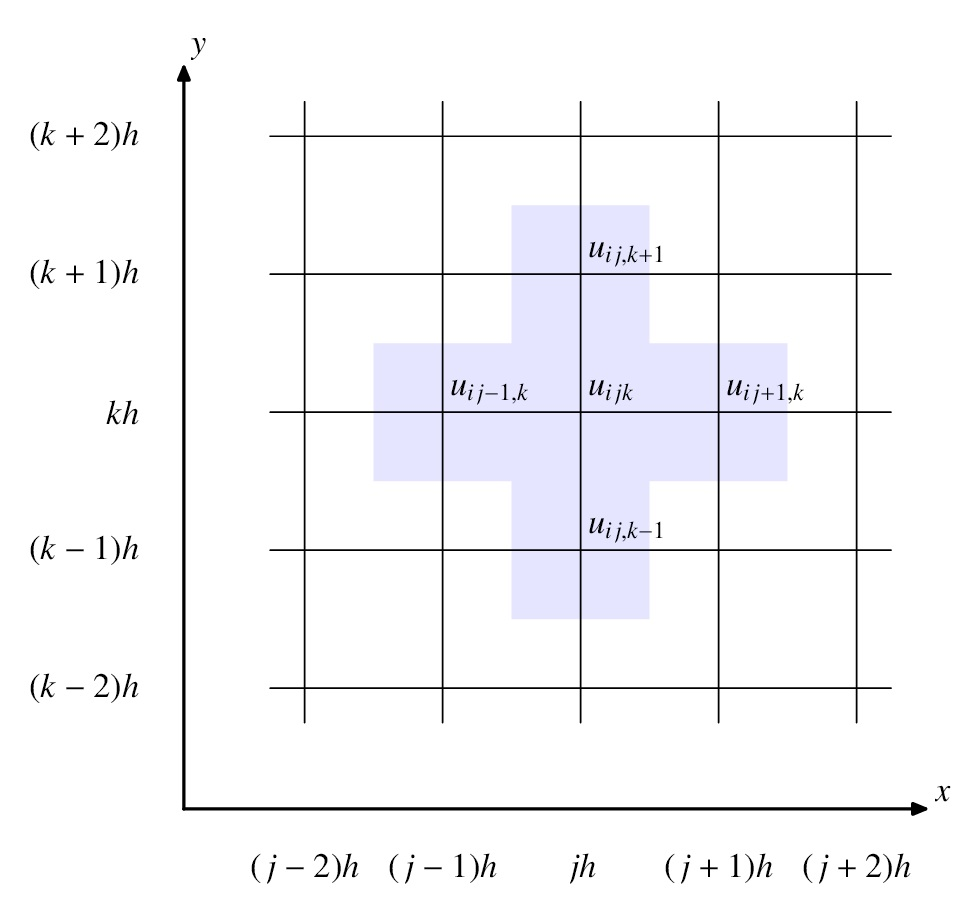
\includegraphics[width=0.5\hsize]{potential/images/diskretisierung/gitternetz.jpg}
\caption{Diskretisierung der Platte\label{potential:gitternetz}}
\end{figure}

Die Grafik zeigt, wie die Platte als Gitter dargestellt
wird. Dabei ist jeder Gitterpunkt mit u$_{i,j}$ beschriftet. Mit $i$ und
$j$ wird der Koordinatenwert der Abszisse und Ordinate beschrieben, je
nachdem wo der gemeinte Gitterpunkt liegt. Mit $h$ wird die Gitterbreite
angegeben. Durch das Verkleinern von $h$ erh\"alt man eine h\"ohere
Aufl\"osung. Jedoch steigt auch der Rechenaufwand, da man mehr Werte
berechnen muss.

\subsection{Numerischer Ansatz}
Nun m\"ochten wir einen numerischen Ansatz entwickeln, damit wir f\"ur
jede Funktion $f$ ein L\"osung finden k\"onnen. Dazu verwenden wir eine
Diskretisation der Ableitungen, wie sie im Motivations-Beispiel von
Kapitel 5 dargestellt wurde. Auf diesem Weg erhalten wir eine lineare
Gleichung:
\begin{eqnarray}\label{eq:gleichung}
\dfrac{1}{h^{2}}\cdot(u_{i+1,j}+u_{i-1,j}+u_{i,j+1}+u_{i,j-1}-4\cdot u_{i,j}) = f(x,y)
\end{eqnarray}
Als letzter Schritt wird diese Funktion nach $u_{i,j}$ aufgel\"ost,
wodurch man auf die gesuchte Gleichung kommt.

\begin{equation}\label{eq:gleichung}
u_{i,j}=\dfrac{-h^{2}\cdot f(i,j)+(u_{i+1,j}+u_{i-1,j}+u_{i,j+1}+u_{i,j-1})}{4} 
\end{equation}
Mit Hilfe dieser Gleichung ist es nun m\"oglich, jedes $u_{i,j}$ zu
berechnen, sofern man dessen unmittelbare Nachbarn kennt. Mit $f(x,y)$
k\"onnen zudem beliebige St\"orfunktionen gew\"ahlt werden. Je nach
dem, welcher Algorithmus verwendet wird, sind unterschiedlich viele
Iterationen notwendig. Verwendet man den Gauss-Seidel-Algorithmus,
so beeinflusst jeder berechnete Wert sofort auch die Berechnung des
Nachbarwerts. Beim Jacobi-Algorithmus werden die Werte jedoch erst am
Ende einer Iteration abgeglichen. Dadurch erspart man sich den Abgleich
innerhalb der Iteration, jedoch berechnet man die Nachbarwerte mit
einem vorhergehenden Wert, wodurch f\"ur die gleiche Genauigkeit mehr
Iterationen notwendig sind.
F\"ur unsere Berechnungen haben wir als Abbruchbedingung eine Verbesserung
kleiner 0.001 festgelegt. Somit gilt:
\begin{equation*}
u^{'}_{i,j} - u_{i,j} < 0.001 
\end{equation*}
Zu beachten ist ferner, dass beim Anlegen der Elektrode sich das Potential
sofort einstellt. Die einzelnen Iterationen stellen demzufolge keinen
zeitlichen Verlauf dar, wie es im Heat-Beispiel der Fall ist. Somit
gilt, dass sobald ein neuer Wert berechnet wurde, der alte aufgrund der
gr\"osseren Abweichung keine Bedeutung mehr hat. 


\section{Programm-Code}	
Unser Programm \texttt{potential}  basiert  weitgehend  auf  dem  Code  des  W"armleitungs-Beispiels. Ge"andert wurden:
\begin{enumerate}
\item Matrixaufteilung
\item L"osungsalgorithmus
\end{enumerate}
Bei der W"armeleitung wird die gesuchte Funktion $u$ abgeleitet. Da
$u$ auch von $t$ abh"angt, tritt die zeitliche Ableitung von $u$ in
der W"armeleitungsgleichung ebenfalls auf. F"ur das Potentialproblem
hingegen reicht eine "ortliche Ableitung. Dies macht die Umsetzung in
Code wesentlich einfacher, was der folgende Codeausschnitt zeigt.
			
	\begin{code}
	// Iterationsausschnitt von iteration.c von heat
		b = -laplacian(u, i,j) - U(u, i, j) / u->ht;	\end{code}	
	
	\begin{code}
	// Iterationsausschnitt von iteration.c von potential
		b = laplacian(u, i, j);	\end{code}	
Ebenfalls wurde der Algorithmus zur Berechnung ge"andert. Dabei wurden
der Jacobi-Algorithmus und der Gauss-Seidel-Algorithmus implementiert,
der zu verwendeter Algorithmus kann beim Start des Programmes ausgew"ahlt
werden. Der grosse Unterschied liegt bei diesen zwei Algorithmen darin,
dass mit den neu berechneten Funktionswerte beim Gauss-Seidel-Algorithmus
weiter gerechnet wird, wohingegen der Jacobi-Algorithmus erst am Schluss
die alten Funktionswerte durch die neuen ersetzt. Dieser Unterschied im
Code sieht folgendermassen aus:
			
	\begin{code}
	// Ausschnitt aus potential_mpi.c fuer den Jacobi-Algorithmus
	if (u->algorithmus == 0)  {
		for (int i = 0; i < udata.length; i++)	{
			udata.u[i] = unew [i];
		}
	}\end{code}
					
	\begin{code}
	// Ausschnitt aus iteration.c fuer den Gauss-Seidel-Algorithmus
	if (u->algorithmus == 1)  {
		u->u[j - 1 + (i -1) * u->width] = unew[j -1 + (i - 1) * u->width];
	}\end{code}	
			
		
\subsection{OpenMPI}	
Wenn die zu berechnende Matrix gen"ugend gross ist, kann eine
Parallelisierung den Rechenvorgang deutlich verk"urzen.

Ebenfalls wird bei einer Parallelisierung die L"osungsmatrix in
Teilbereiche aufgeteilt. Die Anzahl Teilbereiche entspricht dabei der
Anzahl Threads. Dabei m"ussen bei jedem Rechenschritt die Resultate an
den Grenzen der Teilbereiche ausgetauscht werden, damit weiter gerechnet
werden kann. F"ur den Datenaustausch zwischen einzelnen Prozessen,
welche von einander abh"angig sind, ist OpenMPI geeignet und deswegen
wie geschaffen f"ur das Potentialproblem.
				 
	 
\begin{figure}[h] 
\centering 
\includegraphics[width=0.6\hsize]{heat/heat-3.pdf}
\caption{"Ubergabe der Randwerte an den Teilgebietsgrenzen, gleiche Abbildung wie in \ref{potential:domainpartition}}
\end{figure}

Zur Parallelisierung und Verteilung kann die L"osungsmatrix
auf verschiedene Prozesse/Threads aufgeteilt werden. Alle Teilbereiche
haben dieselbe Gr"osse und f"ur jeden Teilbereich ist ein eigener OpenMPI
Prozess zust"andig. 
		
Damit die Daten am Rande der Teilbereiche gesendet werden,
besitzt OpenMPI die Funktion \texttt{MPI\_Send},
welche allerdings nach dem Senden
der Daten blockiert, bis die n"achsten Daten erhalten wurden. Warten
dabei Empf"anger, welche auch Sender sind, in der falschen Reihenfolge
auf die Sender, kann ein sogenannter Deadlocks enstehen. Das heisst, der
Algorithmus bleibt stehen bis der Prozess ein Timeout meldet. Zur Behebung
dieses Problems wurde die Funktion \texttt{MPI\_Isend} verwendet (wie bereits im
Kapitel der W"armeleitung erw"ahnt). Diese Funktion hat den Vorteil,
dass sie Daten sendet und anschliessend weiter arbeitet. Dadurch l"asst
sich ein Deadlock verhindern. 
		
\section{Umsetzung}
Die Problemstellung des Potentialproblems wird mit verschiedenen
Algorithmen gel"ost. Daf"ur werden der Jacobi-Algorithmus und der
Gauss-Seidel-Algorithmus, welche im Kapitel 5 erkl"art wurden,
angewendet. Ebenfalls wurde das Potentialproblem von Andreas Linggi
und Stefan Steiner im Kapitel Visualisierung der Grennschen Funktion
behandelt.

Als Anfangswert diente uns ein FITS-File, welches jeden
Funktionswert $f$ als Pixel darstellt (siehe Input/Output). Die
Zwischenresultate werden anschliessend wiederum als FITS-File ausgegeben,
in welchem jeder Wert der L"osungsfunktion $u$ als Pixel dargestellt
wird.

\subsection{Jacobi-Algorithmus}
Wie auf den Abbildungen sch"on zu erkennen ist, wird bei jedem
Iterationsschritt einen Funktionswertzeile weiter gerechnet. Somit
ergibt sich, dass bei $n$ Dimensionen nach $2n$ Iterationsschritte alle
Funktionswerte berechnet sind. Dies kann man in einem Video, welches aus
allen Rechenschritten zusammengesetzt ist, optisch gut verifizieren. Da
der Jacobi-Algorithmus eine Approximation berechnet, wird sich das
Resultat auch nach $2n$ Iterationsschritte noch geringf"ugig ver"andern,
was von Auge aber nicht mehr ersichtlich ist
(Abbildung~\ref{potential:jacobi}). 

\begin{figure}
\centering 
\subfigure{\includegraphics[width=0.2\hsize]{potential/images/jacobi/0.jpg}}
\quad 
\subfigure{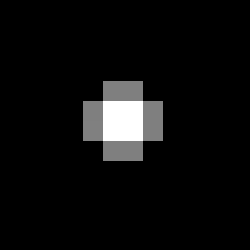
\includegraphics[width=0.2\hsize]{potential/images/jacobi/1.jpg}}
\quad 
\subfigure{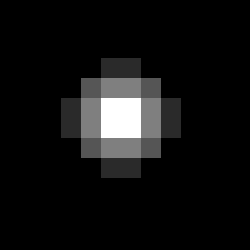
\includegraphics[width=0.2\hsize]{potential/images/jacobi/2.jpg}} 

\centering 
\subfigure{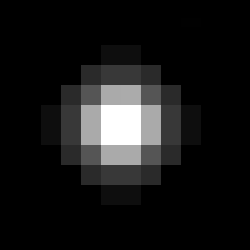
\includegraphics[width=0.2\hsize]{potential/images/jacobi/3.jpg}}
\quad 
\subfigure{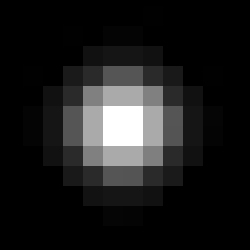
\includegraphics[width=0.2\hsize]{potential/images/jacobi/4.jpg}}
\quad 
\subfigure{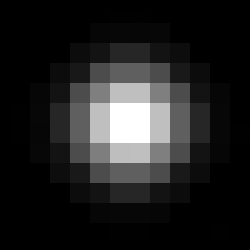
\includegraphics[width=0.2\hsize]{potential/images/jacobi/5.jpg}} 
\caption{Ausgangsbild und die ersten f"unf Iterationsschritte beim
Jacobi-Algorithmus\label{potential:jacobi}} 
\end{figure}


\subsection{Gauss-Seidel-Algorithmus}
Beim Gauss-Seidel-Algorithmus wird, im Unterschied zum
Jacobi-Algorithmus, die neue L"osung direkt verwendet und die
darauffolgenden Funktionswerte von $u$ k"onnen bereits mit
den neuen Werten berechnet werden. Wie in der Bildstrecke gut
ersichtlich, ist die Konvergenz in eine Richtung sehr viel besser
als beim Jacobi-Algorithmus, in die andere Richtung allerdings
nur gleich gut. Dies liegt daran, dass die L"osungsmatrix mit
einer \texttt{for}-Schleife von oben nach unten durchiteriert
wird. Dadurch werden die Funktionswerte auf der rechten Seite,
dass heisst diejenige, welche noch nicht berechnet wurden,
bereits mit dem neuen Wert berechnet. Alle vorhergehenden
Funktionswerte weisen hingegen nur die gleiche Konvergenz wie
der Jacobi-Algorithmus auf. 
	
\begin{figure}
\centering 
\subfigure{\includegraphics[width=0.2\hsize]{potential/images/gs/0.jpg}}\quad 
\subfigure{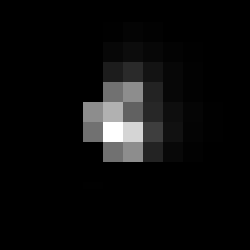
\includegraphics[width=0.2\hsize]{potential/images/gs/1.jpg}}\quad 
\subfigure{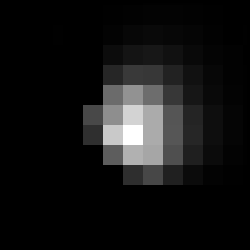
\includegraphics[width=0.2\hsize]{potential/images/gs/2.jpg}} 

\centering 
\subfigure{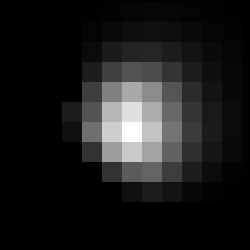
\includegraphics[width=0.2\hsize]{potential/images/gs/3.jpg}}\quad 
\subfigure{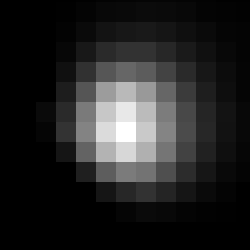
\includegraphics[width=0.2\hsize]{potential/images/gs/4.jpg}}\quad 
\subfigure{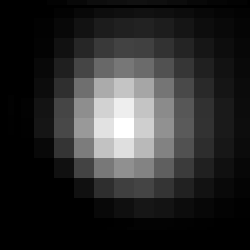
\includegraphics[width=0.2\hsize]{potential/images/gs/5.jpg}} 
\caption{Ausgangsbild und die ersten f"unf Iterationsschritte beim
Gauss-Seidel-Algorithmus\label{potential:gaussseidel}} 
\end{figure}

Die Asymmetrie des Gauss-Seidel-Algorithmus l"asst
sich mit dem symmetrischen Gauss-Seidel-Algorithmus beheben
(im Kapitel SOR behandelt). In unserem Code wechselt dabei die
\texttt{for}-Schleife jedes Mal ihre Richtung. Dadurch ergibt
sich ein "ahnliches Bild wie beim Jacobi-Algorithmus, welches
schneller divergiert. 

\begin{figure}
\centering 
\subfigure{\includegraphics[width=0.2\hsize]{potential/images/sgs/0.jpg}}\quad 
\subfigure{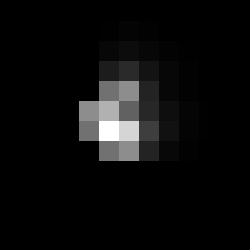
\includegraphics[width=0.2\hsize]{potential/images/sgs/1.jpg}}\quad 
\subfigure{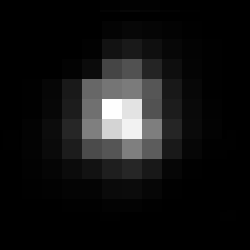
\includegraphics[width=0.2\hsize]{potential/images/sgs/2.jpg}} 
\\
\centering 
\subfigure{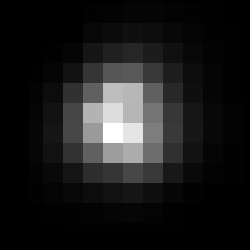
\includegraphics[width=0.2\hsize]{potential/images/sgs/3.jpg}}\quad 
\subfigure{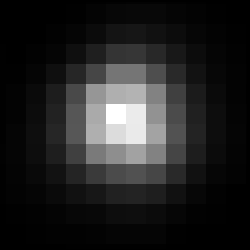
\includegraphics[width=0.2\hsize]{potential/images/sgs/4.jpg}}\quad 
\subfigure{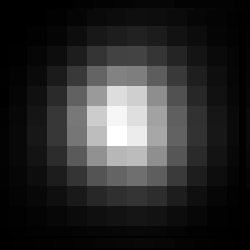
\includegraphics[width=0.2\hsize]{potential/images/sgs/5.jpg}} 
\caption{Ausgangsbild und die ersten f"unf Iterationsschritte beim
symmetrischen Gauss-Seidel-Algorithmus} 
\end{figure}

\subsection{Konvergenz}
F"ur die Ausf"uhrung des Codes kommt es nicht darauf an, welcher
Algorithmus ausgew"ahlt wird. Eine Iteration dauert f"ur jeden
Algorithmus genau gleich lang, allerdings ist die Konvergenz beim
Gauss-Seidel-Algorithmus und beim symmetrischen Gauss-Seidel-Algorithmus
sehr viel besser als beim Jacobi-Algorithmus. Um dies aufzuzeigen,
wurde in den Code eine Abbruchbedingung programmiert. Diese ist erf"ullt,
wenn die maximale Differenz zwischen einem neuen Funktionswert zum alten
Funktionswert einen gewissen Wert unterschreitet.

\begin{center}
\begin{tabular}{ | l | l | l | p{5cm} |}
\hline
\textbf{Algorithmus} & \textbf{Anzahl Iterationen} & \textbf{Berechnungsdauer} \\ \hline
Jacobi-Algorithmus & 570 & 0.3425706 \\ \hline
Gauss-Seidel-Algorithmus & 404 & 0.221811 \\ \hline
symmetrischer Gauss-Seidel-Algorithmus & 405 & 0.22304408\\
\hline
\end{tabular}
\end{center}

\begin{figure}
\centering 
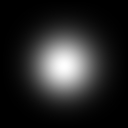
\includegraphics[width=0.6\hsize]{potential/images/konvergenz/konvergenz.jpg}
\caption{Numerische L"osung nach dem das Konvergenzkriterium erf"ullt ist.
Als Input wurden die innersten vier Pixel auf weiss gesetzt, alles andere war
schwarz.}
\label{konvergenz}
\end{figure}

\section{Input/Output}
Als Input wird ein FITS-File verwendet. Dabei werden auf einer schwarzen
Fl"ache (black = 0.0 / 0 \%) Elektroden angelegt (white = 255.00 /
100 \%). Als Output werden ebenfalls FITS-Files verwendet. Je nach
gew"ahlter Einstellung kann die Zwischenl"osung nach $s$ Schritte in
ein FITS-File geschrieben werden. Schlussendlich werden die FITS-Files
in JPEG-Files konvertiert und weiter zu einem MPEG-File verarbeitet. Da
das MPEG-Format verlangt, dass die Bilddimensionen durch 16 teilbar sind,
wurden nur $n\times n$-Bilder untersucht, mit $n = 2^k$, $4\le k\le
12$. S"amtliche verwendeten Shell-Scripts sind auf GitHub einsehbar. 

\section{Resultate}

In diesem Kapitel stellen wir die erhaltenen Messresultate f"ur
Parallelisierungsversuche f"ur die Potentialgleichung vor. Zur L"osung
des Problems wurde wie bereits erw"ahnt OpenMPI verwendet. 
	
\begin{figure}
\centering 
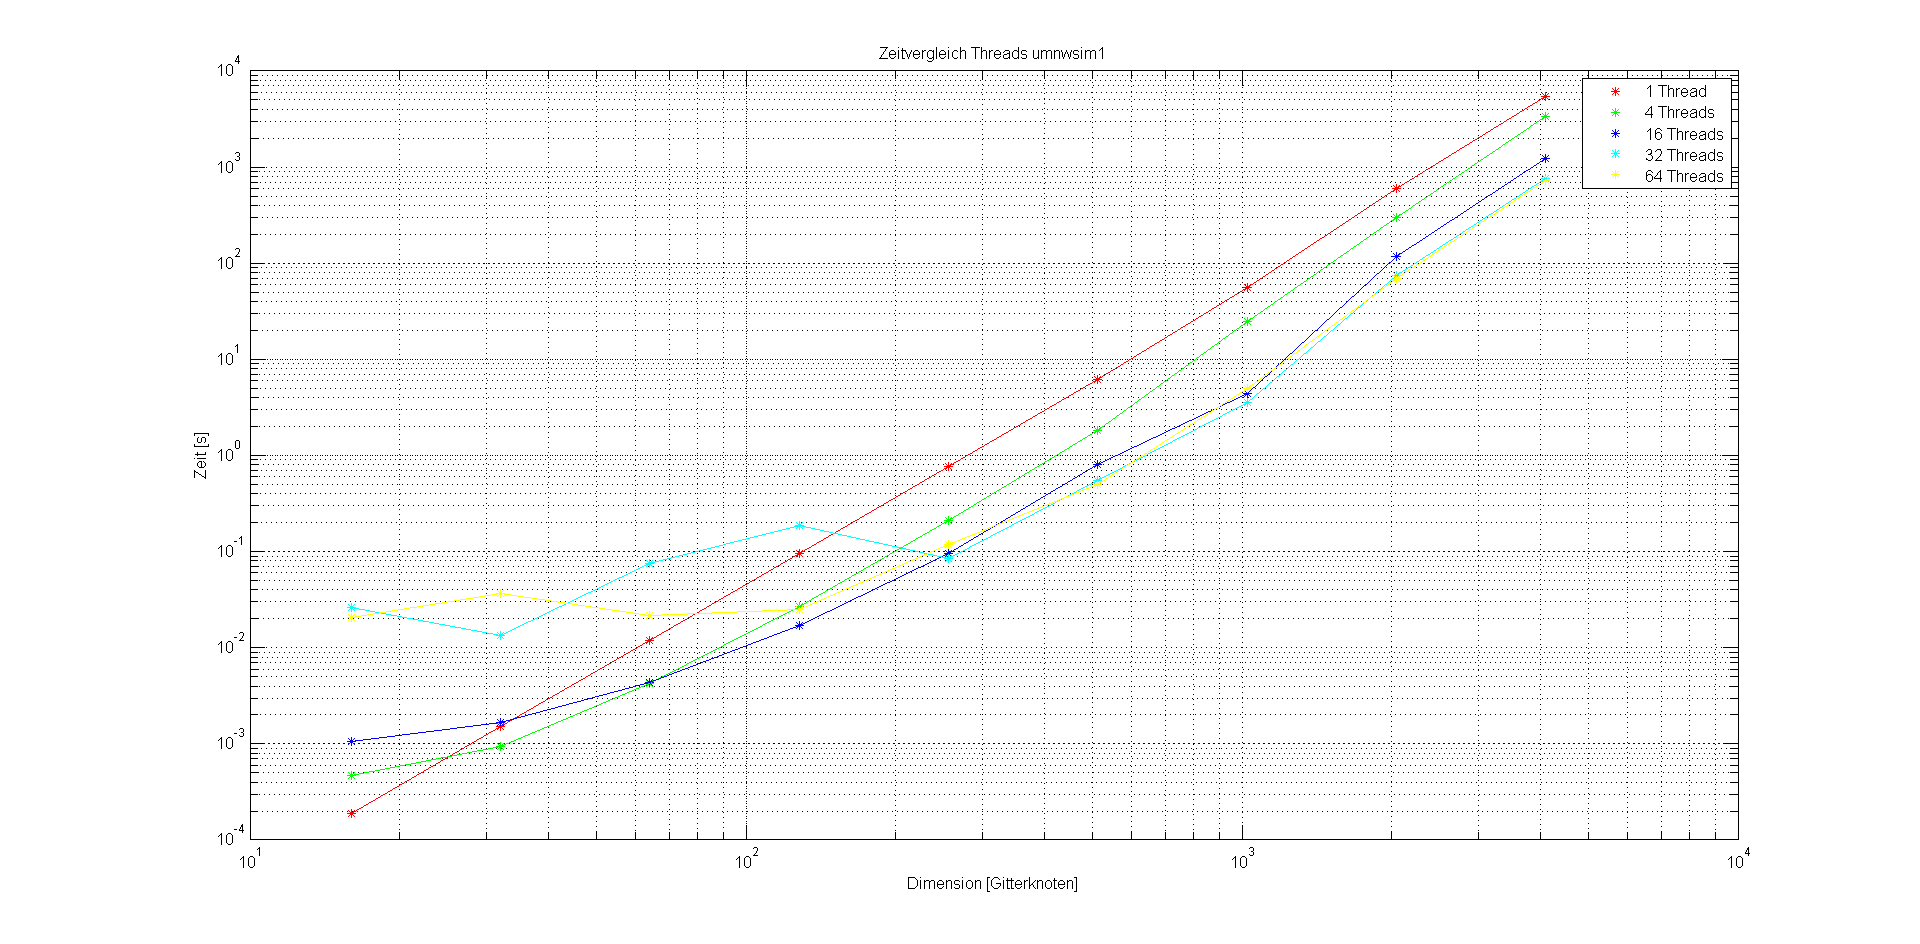
\includegraphics[width=\hsize]{potential/images/Resultate/dimension}
\caption{Laufzeit der mit OpenMPI parallelisierten L"osung}
\label{dimension}
\end{figure}
		
Der Algorithmus wurde mit verschieden grossen Inputs und
verschiedenen Anzahl Threads simuliert. F"ur die Berechnung der L"osung
auf einem $n-dimensionalem$ Gebiet wurden jeweils $2n$ Iterationen
durchgef"uhrt. Beispielsweise wurde einen 1024 x 1024 Input 2048-mal
iteriert, bis der Algorithmus abbrach. In der Abbildung \ref{dimension}
ist jeder Punkt ein Mittelwert von f"unf Messungen. Es wird ersichtlich,
dass sich die Parallelisierung erst ab einer gewissen Gr"osse lohnt. Wird
nur eine kleine Matrix als Input verwendet, ist eine sequenzielle
L"osung mit einem Thread wesentlich schneller und mit weniger Aufwand
verbunden. Dies hat den Grund, dass OpenMPI einerseits initialisiert
werden muss und andererseits unn"otig viele Daten ausgetauscht werden,
obwohl ein einzelner Rechenkern diese mathematische Aufgabenstellung
problemlos berechnen kann. 
	
Beim Simulieren stellte sich allgemein das Problem, dass
bei einem Output bei jedem Schritt die Festplatte stark strapaziert
wurde. Beispielsweise fallen bei einem Input von einem 1024 x 1024
FITS-File und 2048 Iterationen 17.2 GB Daten an. Diese Aktivit"at der
Festplatte verf"alschte die Statistik wesentlich und produzierte eine
grosse Streuung. Die Minimal- und Maximalwerte lagen teilweise mehr als
90 \% auseinander. Aus diesem Grund und auch aus dem Fakt, dass auf dem
HSR-Rechner umnwsim1 nur 40 GB pro User zur Verf"ugung gestellt werden,
wurde der Output g"anzlich unterdr"uckt. Das Ergebnis war anschliessend
konsistent und lieferte kleinere Resultate mit einer sehr kleinen
Streuung. 
	
\begin{figure}
\centering 
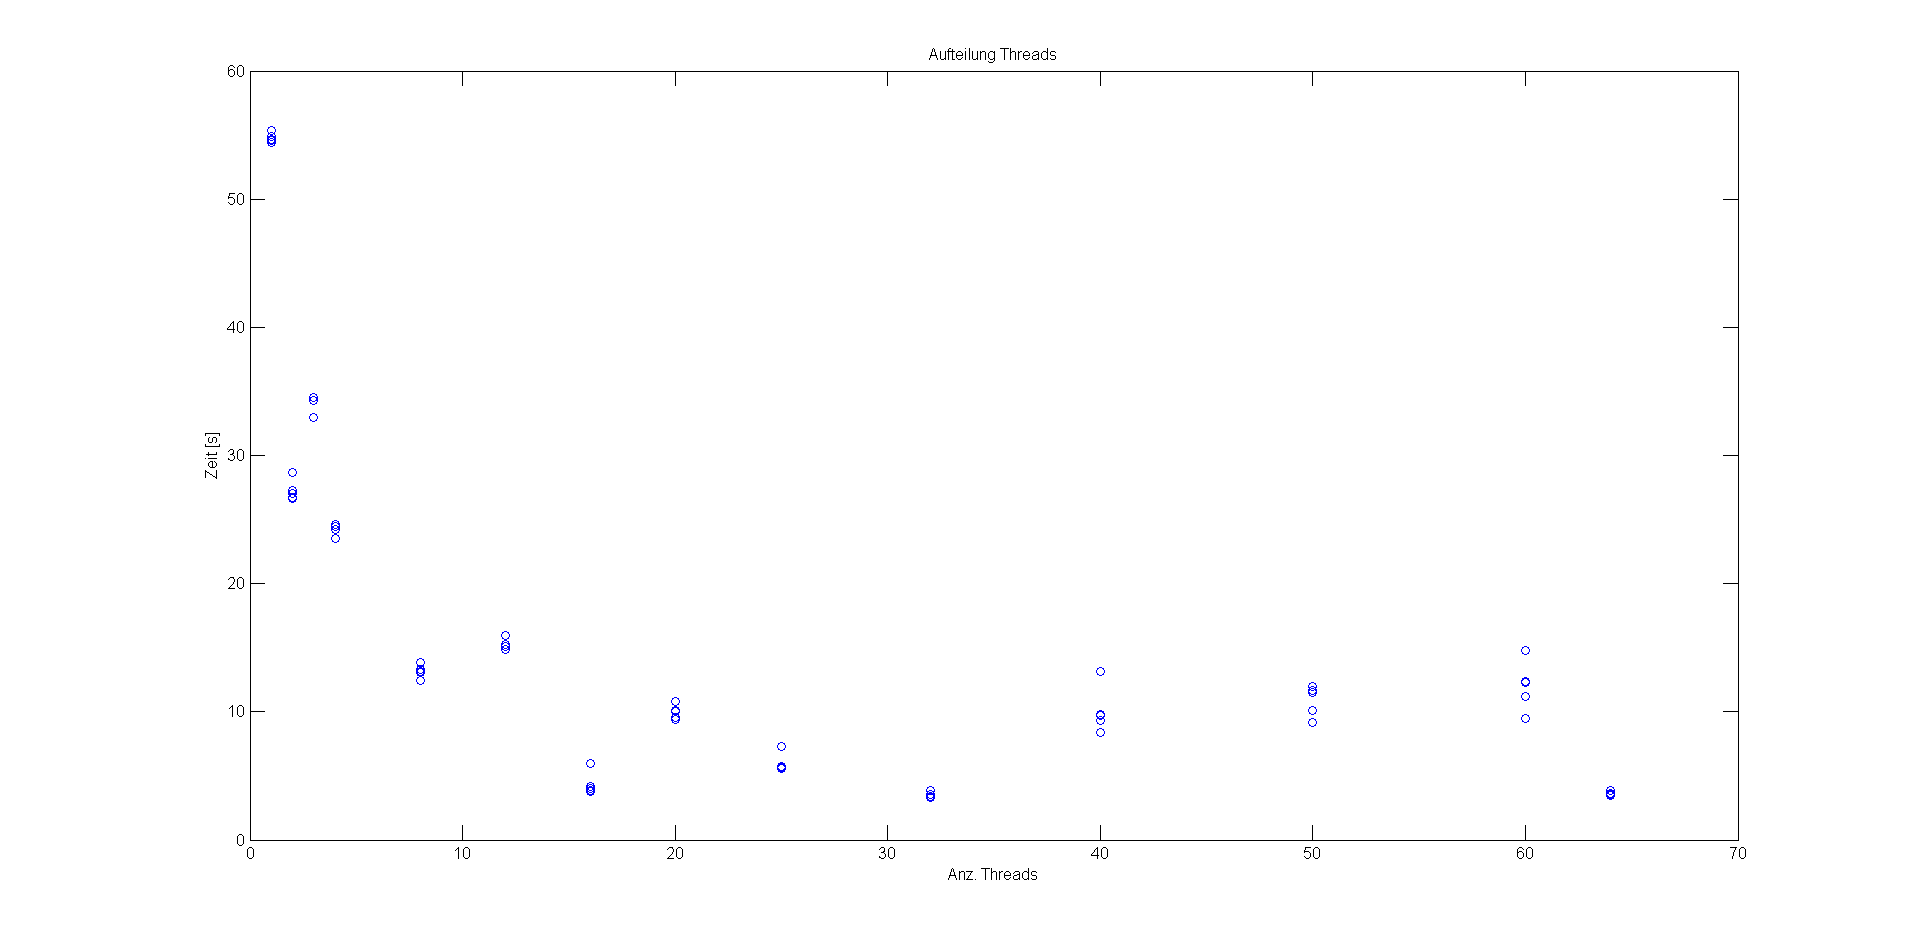
\includegraphics[width=\hsize]{potential/images/Resultate/threads}
\caption{Laufzeit der mit OpenMPI parallelisierten L"osung der
Potentialgleichung in Abh"angigkeit von den Anzahl Threads.}
\label{threads}
\end{figure}

Ebenfalls wurde der Algorithmus mit verschiedenen Anzahl
Threads, daf"ur immer mit der gleichen Aufgabenstellung laufen
gelassen. F"ur diese Simulation wurde einen Input von 1024 x 1024
verwendet und 2048-mal iteriert. Wiederum wurde der Output von
Daten unterdr"uckt. Beim Simulieren mit mehreren Threads wurden auch
verschiedene Aufteilungen eingestellt. Beispielsweise wurden bei 60
Threads vier verschiedene Aufteilungen untersucht, n"amlich 1 x 60,
2 x 30, 3 x 20 und 6 x 10. Es stellte sich heraus, dass sich grosse
Unterschiede erkennen lassen in der Geschwindigkeit des ausgef"uhrten
Algorithmus. Die schnellste Berechnungszeit erh"alt man nicht unerwartet
bei 6 x 10. Dies liegt daran, dass die Matrix $u$ besser aufgeteilt
wird und die zu "ubergebenden Grenzen kleiner werden. Je nachdem wie
der Input gew"ahlt ist, kann es auch einen Unterschied in der Konvergenz
geben. In der Abbildung \ref{threads} ist gut ersichtlich, dass sich ab
ca.~16 Threads keinen wesentlichen Zeitgewinn mehr ergibt. Dies liegt
daran, dass OpenMPI sehr viele Daten "ubertragen muss und die Performance
dadurch nicht mehr ansteigt. Ebenfalls einen Einfluss k"onnte die Hardware
haben. Der HSR-Rechner umnwsim1 hat 32 Cores, infolgedessen brauchen
bei 64 parallelen Threads immer je zwei Thread den gleichen Cache. Dies
ist nat"urlich bei so grossen mathematischen Aufgabenstellungen nicht
sehr hilfreich und kann ebenfalls zu einer Verlangsamung der Simulation
f"uhren. Ob mit 64 Cores wirklich schneller gerechnet werden kann,
konnte nicht ermittelt werden, weil daf"ur die Hardware fehlte.

Die schnellste Rechengeschwindigkeit mit der zur Verf"ugung
stehenden Hardware wurde mit 32 Threads erreicht. Interessant ist, dass
eine Simulation mit 16 Threads nicht wesentlich langsamer ist. Wichtig
ist dabei zu bedenken, dass eine grosse Anzahl Prozessorkerne nicht
nur mehr Geld bei der Anschaffung kosten, sondern auch einen h"oheren
Energiebedarf haben, sei es zum Berechnen oder zum K"uhlen. Deshalb kann
eine Berechnung mit 16 Threads wirtschaftlich g"unstiger sein. 

Diverse weitere numerische L"osungen sind auf GitHub als
MPEG-File verf"ugbar.
	
\subsection{Fazit}
Grunds"atzlich ist gut zu erkennen, dass eine Parallelisierung den Code
wesentlich schneller machen kann, sofern die Parameter richtig eingestellt
werden und bei einem allf"alligen Output auch die verwendete Hardware
gen"ugend schnell ist. Je nachdem wie gross der Input ist, sollte die
Anzahl verwendeter Threads sinnvoll angepasst werden. Dadurch l"asst
sich einiges an Simulationszeit einsparen. 
	
Ebenfalls wurde ersichtlich, dass der Gauss-Seidel-Algorithmus
und der symmetrische Gauss-Seidel-Algorithmus wesentlich schneller als
der Jacobi-Algorithmus sind.
	
	
\end{refsection}
